\documentclass[letterpaper,twoside,11pt,fleqn]{article}

\usepackage[T1]{fontenc}
\usepackage{lmodern}

\usepackage{geometry}
\geometry{letterpaper}

%%% TODO: Add more details about the differences between macros, e.g., for
%%% funcdef2, funcdefna, etc.
%\ifusecolor
\usepackage[pdftex,                             % For PDF output
%              letterpaper,                     % letterpaper no
%              longer supported
              backref,
              baseurl={http://www.mpi-forum.org},
              colorlinks=true,
              filecolor=black,
% for normal and reviewcolors versions:
              linkcolor=blue,
              citecolor=red,
              urlcolor=blue,
% for normal and reviewcolors versions:
% (colorlinks is not changed, to be absolutely sure that all spacing is the same)
%              linkcolor=black,
%              citecolor=black,
%              urlcolor=black,
              hypertexnames=true,
              pdfauthor={MPI-Forum},
              pdftitle={Instructions for Preparing the MPI Standard Document},
              pdfsubject={MPI: A Message-Passing Interface Standard},
              pdfkeywords={Message Passing, MPI, Standard},
              pdfpagelabels,
              plainpages=false
              ]{hyperref}      % For hyperlinks
\usepackage{array}

\def\cmd#1{\texttt{\char`\\#1}}
\def\deprecated#1#2{\ifvmode\else\par\fi The name \cmd{#1} is a
  deprecated alias.  Do not use it and consider replacing it with \cmd{#2}.}
\def\MPI/{\textsf{MPI}}    % MPI macro -- see TEX Book,
\def\MPII/{\textsf{MPI-1}} % MPI-1 macro -- can't easily do MPI1
\def\MPIIVDOTO/{\textsf{MPI-4.0}}
\def\gb{\penalty10000\hskip 0pt plus 8em\penalty4800\hskip 0pt plus-8em%
\penalty10000}
\def\flushline{\hfill\hbox{}\linebreak}

% Uncomment this to help find overfull boxes
%\overfullrule=5pt

\begin{document}
% From the web, the following may make pdflatex conform to the TeX specification
\special{papersize=8.5in,11in}
\setlength{\pdfpageheight}{\paperheight}
\setlength{\pdfpagewidth}{\paperwidth}


\title{Instructions for Preparing the \texorpdfstring{\MPI/}{MPI}
  Standard Document}

\author{Message Passing Interface Forum}

\date{\today}
\maketitle

\section{Introduction}
This document provides guidance on editing the \MPI/ standard
documents.  The \MPI/ standard uses LaTeX, a powerful markup language
where items are marked based on the content, rather than low-level
control of individual formatting options as in WYSIWYG (what you see
is what you get) markup.  LaTeX is a high level interface over TeX, a
powerful and general purpose typesetting language.  LaTeX permits the
use of TeX, which gives it extra power but also makes it easy to
introduce the sort of inconsistent formatting that is the bane of
documents produced with WYSIWYG systems.

Section~\ref{sec:access} covers accessing and editing the document.
Section~\ref{sec:formatting} covers use of markup in the document.
This includes formatting the text and, in Section~\ref{sec:code},
markup used to automate testing of code examples.
Section~\ref{sec:pdf} covers some special considerations for creating
the PDF file for the standard.
Section~\ref{sec:build} covers how to create the document.
Section~\ref{sec:editing} covers the process to be followed in making
changes to the document.
Section~\ref{sec:not-to-do} provides some examples of what \emph{not}
to do in the document.
Section~\ref{sec:choosing-words} discusses some of the subtle issues in
word choices in a standard, such as where to use should and where to
use shall.
Finally, Section~\ref{sec:other} covers topics not discussed elsewhere.

\section{Accessing the Document}
\label{sec:access}

The \MPI/ standard documents are maintained in the git repository
\url{github.com/mpi-forum}.
Instructions on accessing the \MPI/ standard, identifying problems,
suggesting improvements, and creating update candidates to be applied
to the standard may be found in the wiki associated with that
repository.
Those instructions will not be duplicated here.  However, a few
comments here clarify some of the procedures.

It is important, even for the master editor of the document, to follow
both the workflow for updating the document and the style of using
git.
In particular, updates should be small and focused on a single issue.
For example, if while working on an issue, you discover a mis-spelled
word, do \emph{not} fix that mis-spelling.  That should be done as a
separate change, and especially committed as a separate change.  Yes, this is
inconvenient and can cause useful fixes to be lost (because of that
inconvenience), but hard-core git users will object if you don't do
this.

As part of the workflow, changes to the document that are ready to be
applied (and have been approved by the \MPI/ Forum or are considered
minor document changes under the control of the document editor) are
packaged up as \emph{pull requests}.
A pull request is really a set of edits to the \MPI/ standard,
usually created as a branch off of the current state of the \MPI/
standard.
In the recommended workflow, developing this change is done in a
private copy of the repository. This allows the change to be tested
with respect to the current state of the document.  However, most
users are not permitted to commit changes directly back to the
repository.  Instead, the workflow is to push these changes to a
special repository created by the user.  This repository is used for
\emph{nothing} other than communicating the update as a pull request;
in particular, there is no need for this special repository to be
up-to-date, and it \emph{must not} be used to test the update.
Once the pull request is made, the \MPI/ document editor can choose to
apply the pull request, and can follow steps to test the pull request
before applying it.
The workflow for pull requests is documented at
\url{https://github.com/mpi-forum/mpi-issues/wiki/Creating-Simple-Pull-Request}.
Note that pull requests must merge cleanly before an item can be
brought up for a vote.
Instructions for the document editor to test this pull request are
still under construction.

\section{Formatting the Document}
\label{sec:formatting}

For compatibility with the widest variety of editors, text should be
wrapped to fit with 80 columns.  Edits should avoid reflowing text as
this complicates identifying real changes in the document.
The document follows the conventions and spelling of American English.

\subsection{Basic Formatting}

For the most part, text should not use TeX (or LaTeX) formatting
commands.  In particular, font or size changes should not be used.
Formatting of \MPI/ names and C and Fortran code is handled with the
macros defined below.  You may use \cmd{emph} to \emph{emphasize}
text, as in \verb+\emph{emphasize}+, but do not use \cmd{emph} for
formatting terms (discussed later).  The command \cmd{mpicode} may be
used for miscellaneous language-independent code for which there are
no appropriate \MPI/ macros.  The command \cmd{code} should be used
for code in a specific language, such as C or Fortran.
Note that most uses of text font selection, including
``face'' (such as bold or sans serif), are erroneous.  That is, you
should use the appropriate markup for the kind of content, rather than
change the font.  The commands \verb+\textbf+ and \verb+\textsf+
should almost never be used.  See Section~\ref{sec:objects} for the
LaTeX commands to be used with different \MPI/ objects.

TeX has a very sophisticated system for hyphenating words.
However, it will not hyphenate a word that already contains a hyphen.
If you want TeX to hyphenate such a word (e.g.,
implementation-dependent), use \verb+\hyphen/+ instead of the
hyphen, as in
\begin{verbatim}
     implementation\hyphen/dependent
\end{verbatim}
Hyphenation should \emph{never} be used for \MPI/ names.
This is discussed more below.

Spaces \emph{are significant} in LaTeX.  Attempting to make the LaTeX
source look more like a C program (some \MPI/ document authors have done
that) introduces unintended additional spacing that is jarring to the
eye and can
interfere with tools used to find changes in the document.

References to other parts of the standard should use only the section
label; macros to make this relatively easy are described below in
Section~\ref{sec:not-to-do}. They should not also include the page
number, as this is often misleading, since the
page number will refer to the beginning of the section but the typical
use of these is to point to the entire body of the section, which
almost certainly spans multiple pages, or to a specific page within
the section, but not necessarily the first page of the section.
See Section~\ref{sec:not-to-do} for some examples of how to refer
within the document in a way that permits the generation of versions
with and without page numbers.

In a few cases, referring to a page is unavoidable.
For example, you need to refer to a specific advice to users or to an
equation in the text.
In this case, use \cmd{pagelabel} instead of \cmd{label}.
This ensures that any hyperlink will jump to the correct location.
Using just a label may get the correct page number, but the hyperlink will go
to the most recent section or advice/users/rationale environment.

LaTeX defines many environments and many others may be added to
LaTeX.  To preserve a uniform appearance, use only these environments
or the ones specifically defined for the \MPI/ standard in
Section~\ref{sec:mpi-envs}.  Most
of these are well-known; where there is some subtle feature, this is
noted (e.g., between ``center'' and ``centering'').
\begin{description}
\item[array]Use for a tabular layout of data in an equation.
\item[center]This environment should be used to center tables and text
  outside of figures.
\item[centering]This environment should be used to center figures (it
  does not add additional space around the figure).
\item[description]Use for labeled lists. See
  Section~\ref{sec:description} for more on the use of this environment.
\item[displaymath]Use for displayed equations (that is, an equation
  that is separated from the text).
\item[enumerate]Use for numbered lists.
\item[eqnarray]Use for displaying several equations in a single block,
  with each equation lined up with the others (typically at the $=$)
\item[example]This environment should be used for example program
  fragments. See Section~\ref{sec:examples} for more on the use of
  this environment.
\item[figure]Note that captions (with the \cmd{caption} command) go
  below figures.
\item[itemize]Use for unnumbered lists. If list items are full
  sentences, they should be capitalized and end with a period. If they
  are sentence fragments, they should not be capitalized and in many
  cases each item should end with a comma, except the last where a
  period or a comma may be used as appropriate and the penultimate
  item, which should end with ``, and''. E.g., it should have the same
  punctuation as an inline list.
\item[lstlisting]Use for C and Fortran code. See Section~\ref{sec:code}.
\item[obeylines]Use when each newline in the source file should cause
  a new line in the output.  This should only be used in special
  cases, such as a list of contributors.
\item[tabbing]This environment is discouraged; please use one of the
  others, such as \verb+tabular+.  It provides a way to line up
  different columns in a block of text.
\item[table]Note that captions (with the \cmd{caption} command) go
  \emph{above} tables (tables themselves are created with the
  \texttt{tabular} or \texttt{tabularx} environment).
Table placement should use either
  \verb+[tb]+ or (only for large tables) \verb+[p]+.  Never use the
  ``here'' option (\verb+[h]+).

The table environment should \emph{never} be used to create a floating
block of text.
If it doesn't have a caption, do not use the table environment---and
don't add a caption just to get around this.
Consult the document editor if you feel you need to create a floating
block of text.

\item[tabular]Used to create tables. Use \cmd{textbf} for headings; use
 \cmd{hline} only on the top, bottom, and after then heading. In some case,
 \cmd{hline} may be used to separate blocks of items.
\item[tabularx]An enhanced version of \verb+tabular+, it includes a new
column type, \verb+X+, that provides an automatically-sized column for a
paragraph of text.
See \url{http://ctan.math.utah.edu/ctan/tex-archive/macros/latex/required/tools/tabularx.pdf}\flushline
for more information.
\item[verbatim]Use this for the rare cases where fixed-width text is
  required, and for code examples that cannot use \verb+lstlisting+
  (see more below on special
requirements for code) and for other fixed-width text.  For example,
this is often used in the text to show the code for two processes side
by side.  If a \verb+verbatim+ is \emph{not} used for a code example,
it must be prefixed with
\begin{verbatim}
%%HEADER
%%SKIP
%%ENDHEADER
\end{verbatim}
This keeps the tool that checks the code examples from trying to
compile the contents of the \verb+verbatim+.
\item[Verbatim]An alternative form of verbatim that allows the use of
  TeX commands within the Verbatim environment.  Note that this should
  \emph{not} be used for code examples, as it interferes with the automated
  checks that tests that the code examples compile.
\end{description}

To include a graphic image, use \cmd{includegraphics}.  This command
can rescale the size of the image.  A typical use (from the
Collectives chapter) is
\begin{verbatim}
    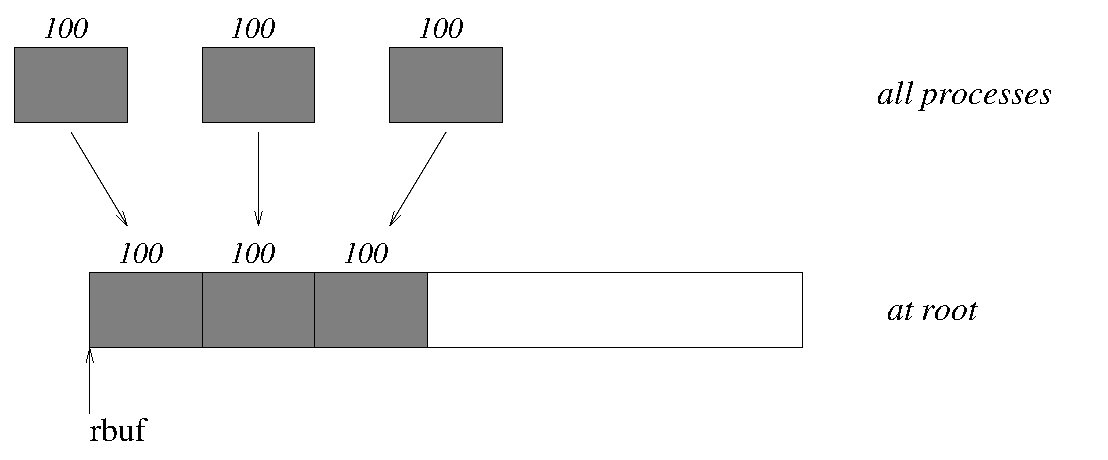
\includegraphics[width=4in]{figures/mycoll-fig2}
\end{verbatim}
Figures should be provided in PDF (\texttt{pdf}) format.  Figures
should be placed in the \texttt{figures} directory, not in the
chapter's directory.

Explicit linebreaks should be avoided unless they are used where a
linebreak is always required, such as at the end of a line of
declarations. Use \cmd{gb} (for ``good break'') to tell LaTeX where
it may be better to break a line.  The reason for using this is that
if subsequent edits to the text change the flow of the paragraph, the
line breaks will be adjusted accordingly.  If \cmd{gb} doesn't work
(it uses TeX linebreak penalties to suggest a good spot at which to
break the line, but does not force it), try \cmd{vlgb}.  This is a
version of \cmd{gb} that may add a larger amount of whitespace to the
line, making a break there more likely.

In cases where you need to force a linebreak, use \cmd{flushline}.
This ensures that the line is broken at that point, and that the line
is \emph{not} right justified.

Because \MPI/ names (e.g., function names, constants, objects) are
long and never hyphenated or broken across a line, TeX may be unable to
find a good set of line breaks and/or line spacing, resulting in
either overfull lines (names extending right into the margin) or very
poor spacing between words.
In this case, use \cmd{flushline} to force a line break; the line
will \emph{not} be right justified.
This is not a perfect solution, but it is less ugly than the
alternatives, and avoids any confusion over whether a dash
(\texttt{-}) is part of the name of an \MPI/ term.
An example of the use of \cmd{flushline} in this case is shown
below, taken from the Datatype chapter:

\begin{verbatim}
In Fortran, the functions
\mpifunc{MPI\_TYPE\_CREATE\_HVECTOR},\flushline  % force break
\mpifunc{MPI\_TYPE\_CREATE\_HINDEXED},
...
\end{verbatim}

References to section, table, figure, or enumerated list items should
not use the number that appears in the document.  Instead, they should
make use of the LaTeX command \cmd{label} and \cmd{sectionref} or
\cmd{ref}.  The
\cmd{label} command creates a symbolic label for the most recent
command that creates a number.  For example,
\begin{verbatim}
  \section{Communication Calls}
  \label{sec:onesided-putget}
\end{verbatim}
creates the label \texttt{sec:onesided-putget}.  This section can then
be refered to with the \cmd{sectionref} command:
\begin{verbatim}
  \sectionref{sec:onesided-putget} describes the ...
\end{verbatim}
The command \cmd{sectionref} will output the text ``Section'' followed
by the section number, including the TeX commands to avoid splitting
the section name and number across a line.
The \cmd{label} command may also be used after a \cmd{caption} command
to get the number of a figure or table, and after the \cmd{item}
command in an enumerated list to get the number of that item.  This
approach is used in the One-Sided Communications chapter to refer to
the different RMA rules.  Using the \cmd{label} and \cmd{sectionref} or
\cmd{ref} commands
ensure that the references remain correct even if a new numbered item
is inserted into the document.

When referencing another part of the document, refer to a section.
For example, use
\begin{verbatim}
Consider the code fragment in Example~\ref{ex:1sided-fence}.
\end{verbatim}
Note the use of the tie (\verb+~+) between the name and the use of
\verb+\ref+. This prevents TeX from breaking the line between the
``Example'' and the example number.  It is \emph{incorrect} to leave
out the tie.

Previous versions of the standard sometimes also provided the page
number; while that is somewhat helpful for printed copies, the section
information is adequate and many users will use on-line versions,
where the section reference will provide a direct link to the relevant
page.  Rather than use inconsistent style, the text standard is to
only use the Section number (and similarly for all other cross
references).
Do not use the section name either.

To make it easy to produce the correct output and to provide the
option of including page numbers, use the following macros:

\begin{center}
\begin{tabular}{|l|l|}\hline
\textbf{Instead of}&\textbf{Use}\\\hline
\verb+Section~\ref{secname}+&\verb+\sectionref{secname}+\\
\verb+Annex~\ref{secname}+&\verb+\annexref{secname}+\\
\verb+Sections~\ref{s1} to~\ref{s2}+&\verb+\sectionrange{s1}{s2}+\\
\verb+Example~\ref{exname}+&\verb+\namedref{Example}{exname}+\\\hline
\end{tabular}
\end{center}
The macro \cmd{namedref} should be used for references with other
names, such as the last one in the list above that shows how to refer
to an Example.

There is one exception to the rule to not use section
names. \cmd{subsubsection} and \cmd{paragraph} are not numbered and a
\cmd{ref} (or \cmd{sectionref}) will not produce the correct label (it
will refer to the number of the enclosing \cmd{subsection}).
In these cases, use \cmd{nameref} to get the name of the
\cmd{subsubsection} or \cmd{paragraph}.

%% Need an ``onpage'' that works for page references to multiple
%% sections.

\subsection{Page references in the Change-Log}
\label{sec:change-log-pages}
The change log requires special care.
Because the change log includes
changes from all versions of the \MPI/ standard, there is a real risk
that references that use symbolic label names that are correct in one
version will become incorrect in a subsequent version.
Page references should be avoided; if necessary, they should refer to
specific official version of the standard.

\subsection{Describing a Change-Log entry}
\label{sec:change-log-entries}
A change-log entry should be a short description of the change. It
should \emph{not} repeat the change.  For example, including an
``advice to implementors'' in the change log is incorrect.  Rather,
the text should point to the change. Note that this may need to point
to a specific page in line \emph{in a specific version} of the
standard.

\textbf{Note that many entries violate this.  See, for example, the
  entry \#32, 17.1.19 on type\_create\_f90\_xxx}.

This is essential, as only the standard text is definitive.  The
change-log should only be used to provide a short summary for readers
interested in the changes, not the exact details.  Readers must be
encouraged to read about the change in the context of the change, not
the short summary in the change log.

\subsection{Descriptions of Terms and \texorpdfstring{\MPI/}{MPI} Objects}
\label{sec:description}
The description environment should be used in most cases where one or
more terms or \MPI/ objects or constants are being described with more
than a few words. For example,
\begin{verbatim}
\begin{description}
\item[\infokey{no\_locks}]If set to \mpicode{true} ...
\item[\infokey{accumulate\_ordering}]Controls the ordering of ...
\end{description}
\end{verbatim}
Note the use of the \verb+\item[name]+ form. It is incorrect to use
\verb+\item{name}+ in a \texttt{description} environment.

In the special case of a list of constants with very short
descriptions, the \texttt{constlist} environment may be used.
For example
\begin{verbatim}
\begin{constlist}
\noconstitem{Name}{Meaning}
\constitem{MPI\_MAX}{maximum}
\constitem{MPI\_MIN}{minimum}
\constitem{MPI\_SUM}{sum}
...
\end{constlist}
\end{verbatim}
\cmd{constitem} is a macro that uses \cmd{mpiconst} in for the first
argument (thus ensuring that the item is indexed properly and in the
correct font). This is built on the LaTeX list environment.
While the \cmd{item} command can be used for list headings and other
lines that don't define a constant, \cmd{noconstitem} ensures that the
output is properly formatted and should be used if possible.
In some cases, two or three constants are needed in the list; for
these cases, use \cmd{constitemtwo} and \cmd{constitemthree}
respectively.
This is shown in this example:
\begin{verbatim}
\begin{constlist}
...
\constitemtwo{MPI\_MAX}{MPI\_MIN}{C integer, Fortran integer,
         Floating point,}
\end{constlist}
\end{verbatim}
In some cases, a list of constants is presented with no description.
For these, use \gb\cmd{constitemonly}:
\begin{verbatim}
\begin{constlist}
...
\constitemonly{MPI\_MAX\_INFO\_KEY}
...
\end{constlist}
\end{verbatim}
If very long (or very short) constant names are used, the width of the
space used for the constant name may be changed with an optional
argument to the environment.  The value of this argument is the width
of the space for the constant names.
For example, the terms chapter uses this:
\begin{verbatim}
\begin{constlist}[200pt]
\constitemonly{MPI\_MAX\_PROCESSOR\_NAME}
...
\constitem{MPI\_ASYNC\_PROTECTS\_NONBLOCKING}{(Fortran only)}
\end{constlist}
\end{verbatim}

The \cmd{paragraph} command should only bee used for headings that are
below that of a \cmd{subsubsection}.
The current (as of \MPIIVDOTO/) version of the standard still uses
\cmd{paragraph} for a general low-level heading and as a way to format
items that should really be in a description or constlist
environment.
Unless the expectation is that a \cmd{paragraph} heading could appear
as a numbered item in the table of contents, it should always be used
in the \cmd{paragraph*} form.
In that case, it \emph{must} be within the scope of a
\cmd{subsubsection}.
In cases where a paragraph heading is desired, but it is not logically
below a \cmd{subsubsection}, the command \cmd{paraheading} should be
used instead of \cmd{paragraph}. This is used in the document as of
\MPIIVDOTO/.

Do not use an en- or em-dash in formatting a list of terms or
names; use the description environment as shown above.

\subsection{Presenting Examples}
\label{sec:examples}
Examples should be presented in the example environment, beginning
with a short description of the example.
Short entries for the example should be included as well.
For example:

\begin{verbatim}
\begin{example}
One sentance description of example.
\Exindex[optional description for list of examples]{language}{short
description for index}{MPI names}
\exindex{other example index entry}
....
\end{example}
\end{verbatim}

The ``language'' in \cmd{Exindex} may be either \texttt{C},
\texttt{Fortran}, or \texttt{Neutral}.
It may also be a list of these languages, with names separated with a comma as
in \texttt{C,Fortran}.
The name \texttt{Neutral} is used for language-independent examples,
including examples for which the programming language used is not clear.
The ``names'' may be a single name or a comma-separated
list of names. Typically, these are \MPI/ routine names, but other
names may be included with a special prefix, as noted below.
The ``short description'' should be just a few words, as it will
appear in the index (if that feature is selected---it currently is not).
\cmd{Exindex} \emph{must} be used within an \texttt{example}
environment.
The ``names'' option may contain any of the following:
\begin{description}
\item[\MPI/ routine names]E.g., \texttt{MPI\_Init}
\item[\MPI/ Declarations]E.g., \texttt{MPI\_Aint}, expressed as
  \texttt{d:name}, e.g., \texttt{d:MPI\_Aint}
\item[\MPI/ Constants]E.g.,\texttt{MPI\_COMM\_WORLD}, expressed as
  \texttt{c:name}, e.g., \texttt{c:MPI\_COMM\_WORLD}
\item[\MPI/ Callback Typedefs]E.g., \texttt{MPI\_Handler\_function},
  expressed as \texttt{t:name}, e.g.,\flushline
  \texttt{t:MPI\_Handler\_function}
\end{description}
For example,
\begin{verbatim}
\begin{example}
This is a example with \mpifunc{MPI\_Send}.
\Exindex{C}{Send and Receive}{MPI_Send,MPI_Recv,c:MPI_COMM_WORLD}%
\end{verbatim}
The ``optional description for list of examples'' is used to provide
the description for the list of examples. If this is not provided, the
``short description'' is used.
This optional argument should always be used if the short description
includes index commands ``!'' or ``@''. For example
\begin{verbatim}
\Exindex[Fortran 90, with datatype]{Fortran}{Fortran 90!with datatype}{}
\end{verbatim}
Only one \cmd{Exindex} command should be used in any Example.

The \cmd{exindex} command was used for \MPI/ versions through
\MPI/-3.1, and was the only command for adding to the Examples index.
The \cmd{Exindex} command has been added for
\MPI/-4.1 in order to improve the value of the indices.
You can continue to use \cmd{exindex} for the cases where an entry is
desired in the examples index without naming an MPI function.
The \cmd{Exindex} command adds entries to both the Examples index and
the MPI Function index.
Uses of \cmd{exindex} that just list an \MPI/ function should be
changed to use \cmd{Exindex}.

See Section~\ref{sec:code} for code examples (within this example
environment) and Section~\ref{sec:mpi-code} for language-independent
examples.
The example environment should be used for code examples, for
examples that illustrate the behavior of \MPI/ routines, and for other
examples within the document.
Do not use \cmd{paragraph} or other ad hoc LaTeX formatting for
examples; unfortunately, there are such uses in the \MPI/-1 through
\MPI/-3.2 documents.

\subsection{\texorpdfstring{\MPI/}{MPI} Environments}
\label{sec:mpi-envs}
There are several environments that are used for special comments to
the reader (advice to user, implementors, and rationale) and for lists
of constants and functions.
\begin{description}
\item[constlist]A list of \MPI/ constants, with a short description of the
  constant. For lists of \MPI/ constants with longer description of
  the constant, use the \texttt{description} environment.
\item[funcdef]The environment used for many \MPI/ function
  definitions.  There are related environments \texttt{funcdef2} (to
  force a line break in the argument list between the first and second
  arguments) and
  \texttt{funddefna} (for functions with no
  arguments). \texttt{funcdef} takes one argument, which is the
  language-independent declaration (complete with arguments), followed
  by one or more \cmd{funcarg} arguments that define each parameter.
\item[implementors]Advice for implementers
\item[mpicodeblock]Used for language-independent code examples
\item[mpi-binding]This is used to describe an MPI binding.  The
  contents of this environment are processed by a separate python
  program, creating a new file that contains the LaTeX commands for
  the function bindings.
  For example, \texttt{pt2pt.tex} is processed to create
  \texttt{pt2pt-rendered.tex}, which is used to create the \MPI/
  standard document.
\item[rationale]Rationale for a choice in the \MPI/ standard.
\item[users]Advice for user
\end{description}

\subsection{\texorpdfstring{\MPI/}{MPI} Objects}
\label{sec:objects}

There are special macros that aid in formatting and automatically
indexing MPI items, such as functions, constants, and strings, as well
as language-specific items, such as C or Fortran datatype names for
types defined by MPI (such as \textsf{MPI\_Status}.

Each of these macros has a base form, which will format the argument
and add it to the appropriate index.
Variaions of these are defined following a regular pattern:
\textsf{\textless{}basename\textgreater[short][main][index\textbar{}skip]}.
The suffix names have the following effect
\begin{description}
\item[short]Use when the argument name is short, \emph{and} when the
  use of the command causes an unsightly line break. These macros do
  \emph{not} use the \cmd{gb} command to allow linebreaks before the
  name.
\item[main]Use when this use \emph{defines} the name---this creates an
  index entry that identifies this use as the location where the name
  is defined.
\item[index]Use to index the name \emph{only}. The term will not be
  formatted into the document.
\item[skip]The opposite of the index option, this does not include the
  name in the index. These are used to add a name without indexing the
  name. This is typically used to format partial names or names with
  \textsf{XXX} (used as a ``wildcard'' for some routine descriptions).
\end{description}
For example, \cmd{mpifunc} is used for language-independent references
to MPI funcations, such as
\verb+\mpifunc{MPI_Send}+. \cmd{mpifuncskip} only adds the name to the
MPI Function index, as in \verb+\mpifuncskip{MPI_Send}+.
Not all combinations are defined for all basenames, and not all
combinations make sense.
The suffixes \texttt{index} and \texttt{skip} are mutually exclusive,
as are \texttt{main} and \texttt{skip}.
If you need a combination that is not currently supported, contact the
document editor.

The base commands are shown in Table~\ref{tab:mpiobjects}.

\begin{table}
\caption{Commands for formatting and indexing MPI names.}
\label{tab:mpiobjects}
\begin{tabular}{>{\raggedright}p{1.5in}|l|>{\raggedright\arraybackslash}p{2.5in}}
\textbf{Object Type}&\textbf{Macro Base Name}&\textbf{Notes}\\\hline
MPI Function&\cmd{mpifunc}&MPI language-independent function
names. Indexes function name in the MPI Function index. Name
\emph{must} be in all uppercase\\
C Function &\cmd{cfunc}&Functions in the C binding for MPI\\
Fortran Function&\cmd{ffunc}&Functions in the Fortran binding for MPI\\\hline
MPI parameter&\cmd{mpiarg}&Parameters used in the description of an
MPI routine\\
C parameter&\cmd{carg}&Parameters used in the C binding of an MPI
function\\
Fortran parameter&\cmd{farg}&Like \cmd{carg}, for Fortran.\\\hline
MPI datatype&\cmd{mpidtype}&MPI Datatype handles\\
MPI callback name&\cmd{mpicallback}&For language-independent names\\
MPI callback type&\cmd{mpiccallbackdef}&For C function
declaration typedef for MPI callbacks, e.g.,
\textsf{MPI\_Comm\_copy\_attr\_function}\\
MPI-defined C type&\cmd{mpictype}&For types such as
\textsf{MPI\_Aint}\\
MPI-defined Fortran type&\cmd{mpiftype}&For types such as
\textsf{TYPE(MPI\_Status)}\\
MPI-defined Fortran kind type&\cmd{mpiftypekind}&For types such as
\textsf{INTEGER (KIND=MPI\_OFFSET\_KIND)}\\\hline
C type&\cmd{ctype}&For C language types, e.g., \texttt{double}\\
Fortran type&\cmd{ftype}&For Fortran language types, e.g.,
\texttt{INTEGER}\\\hline
MPI info key&\cmd{infokey}&For info key strings\\
MPI info value&\cmd{infoval}&For info key values\\
MPI error code&\cmd{error}&For predefined MPI Error codes and
classes\\
MPI string&\cmd{mpistring}&For string values defined by MPI\\
MPI function constant&\cmd{mpiconstfunc}&For predefined functions such as
\textsf{MPI\_COMM\_DUP\_FN}\\
Other MPI constant&\cmd{mpiconst}&For items such as assert values
(\textsf{MPI\_MODE\_NOSUCCEED}), keyvals, split types, and the like\\\hline
\end{tabular}
\end{table}

The command \cmd{mpiconst} is a special case.
It takes an optional argument that specifies the font size, and can be
used to specify the use of a smaller font.
For example, \verb+\mpiconst[1]{MPI_SUCCESS}+ formats
\textsf{MPI\_SUCCESS} with a font size one smaller than the
default.\footnote{Defining this to use an integer for how many steps
  smaller avoids the use of an explicit font size, which could cause
  problems if the default font size were ever changed.}


Occasionally, the standard uses a shorthand to describe a number of
similar functions, as in \textsf{MPI\_FILE\_IXXX}.   Use the
command \cmd{XXX/} to indicate the \textsf{XXX} as in
\begin{verbatim}
    \mpifunc{MPI\_FILE\_I\XXX/}
\end{verbatim}
this ensures that a
consistent style is used in the document.
Do not use $\ldots$ for this purpose.

\subsubsection{MPI Object Examples}
This section provides a few examples of the use of the MPI Object
macros.

MPI functions in the language-independent binding are always in
uppercase, as in \verb+\mpifunc{MPI\_BCAST}+.
To refer to an argument of an MPI function in the language-independent
binding, use \cmd{mpiarg} as in \gb\verb+\mpiarg{array\_of\_handles}+.
A short argument name may be refered to with \verb+\mpiargshort{n}+,
but should only be used when the \cmd{mpiarg} command caused a
unsightly line break.
MPI Datatypes use \gb\verb+\mpidtype{MPI\_DOUBLE}+. MPI C language types,
such as \textsf{MPI\_Aint}, use \gb\verb+\mpictype{MPI\_Aint}+.
MPI Fortran language types, such as \textsf{TYPE(MPI\_Status)}, use
\verb+\mpiftype(MPI\_Status)}+.
A special case is the ``kind types,'' such as
\gb\texttt{INTEGER(KIND=MPI\_OFFSET\_KIND)}.
These use \gb\verb+\mpiftypekind{OFFSET}+.

\subsubsection{NULL used in text}
The term ``NULL'' is used in several different ways in the standard.
Use the following for each type of use:
\begin{description}
\item[Null pointer]Use \verb+\code{NULL}+
\item[Null \MPI/ Object]Use \verb+\mpiconstskip{NULL}+. For specific \MPI/
 objects, use that objects name, e.g., \verb+\mpiconst{MPI_COMM_NULL}+.
\end{description}

\subsubsection{true and false used in text}
When used in the context of the language-independent routines, the
values \textsf{true} and \textsf{false} should be written as
\verb+\mpicode{true}+ and \verb+\mpicode{false}+ respectively.
It is incorrect to use any version of \cmd{const} or \cmd{mpiconst}
for these values.

\subsection{\texorpdfstring{\MPI/}{MPI} Terms}
\label{sec:terms}
The \MPI/ document introduces a number of terms, such as ``message''
and ``send buffer.''
These should be marked as \verb+\mpitermdef{message}+ where the term
is first used and defined, and as \verb+\mpiterm{send buffer}+ at
subsequent uses.  These macros will generate an index entry for each
use, as well as formatting the term in \textbf{bold} for the
definition use (\cmd{mpitermdef}) and in \emph{italics} for other uses
(\cmd{mpiterm}).
Use \cmd{mpitermni} where the term should not be indexed but be
properly formatted in the text.
Use \cmd{mpitermindex} to add an index entry for a term \emph{without}
adding the term to the text; this is appropriate for adding a more
specific index entry for a term.
For example, this text is used in the Point-to-point chapter to
add an index entry for send/receive operations:

\begin{verbatim}
Initiate a nonblocking communication request for a
\mpitermni{send and
receive}\mpitermindex{send-receive!nonblocking} operation.
\end{verbatim}
Note that the \cmd{mpitermindex} immediately follows the
\cmd{mpitermni} command---this is important, as extraneous spaces will
be inserted into the PDF otherwise.

Some chapters have used \textbf{bold} and/or \emph{italics} for terms
and concepts.
These should be changed to use \cmd{mpiterm} and \cmd{mpitermdef} as
appropriate.
In some rare cases, it may not make sense to use the \cmd{mpiterm}
commands. In this case, a term should be formatted in bold with
\cmd{textbf} when first introduced. Subsequent uses should remain in
the same font; i.e., use neither \cmd{textbf} nor \cmd{emph}.

A special case is index entries for terms that refer to section
titles.
These are formatted in \textbf{boldface} in the index, and the
commands are placed immediately after the section commend.
\begin{description}
\item[\cmd{mpitermtitleindex}]Add the name to the term index, with the
  page number in bold face.
\item[\cmd{mpitermtitleindexsubmain}]Adds two entries, a main entry
  that concatenates the two arguments, and a second entry, with the
  first argument a sub-entry to the second argument.
For example,
\begin{verbatim}
\mpitermtitleindexsubmain{Point-to-Point}{Communication}
 results in:
                 Point-to-Point Communication, 23
                 Communication,
                    Point-to-Point, 23
\end{verbatim}
(page numbers are in boldface).
\item[\cmd{mpitermtitleindexmainsub}]Similar to
  \cmd{mpitermtitleindexsubmain}, but the second argument is shown as a
  sub-entry of the first argument and as a top-level entry.
For example,
\begin{verbatim}
\mpitermtitleindexmainsub{Message}{Envelope}
 results in:
                 Message
                    Envelope, 27
                 Envelope, 27
\end{verbatim}
(page numbers are in boldface).
\end{description}

\subsection{Standard Names}
\label{sec:standard-names}

The macros in Table~\ref{tab:mpinames} ensure that the name ``MPI'' is
in the proper font and size.
The \verb+/+ that follows the name is used to ensure that spaces are
preserved (otherwise, TeX removes the blanks after a TeX command from
the output).

An example usage is\\
\verb+It is highly desirable that \MPI/ not use...+\\
will appear as\\
It is highly desirable that \MPI/ not use...

\begin{table}
\caption{Macros to properly format different versions of the \MPI/
  standard.}
\label{tab:mpinames}
\begin{center}
\begin{tabular}{ll} %p{2.5in}}
\textbf{Command}&\textbf{MPI Version}\\\hline
\cmd{MPI/} or \cmd{mpi/}&\MPI/ (no specific version)\\
\cmd{MPIIV/} or \cmd{mpiiv/}&\MPI/-4\\
\cmd{MPIIVDOTO/} or \cmd{mpiivdoto}&\MPI/-4.0\\
\cmd{MPIIII/} or \cmd{mpiiii/}&\MPI/-3\\
\cmd{MPIIIIDOTI/} or \cmd{mpiiiidoti/}&\MPI/-3.1\\
\cmd{MPIIIIDOTO/} or \cmd{mpiiiidoto/}&\MPI/-3.0\\
\cmd{MPIII/} or \cmd{mpiii/}&\MPI/-2\\
\cmd{MPIIDOTO/} or \cmd{mpiidoto/}&\MPI/-1.0\\
\cmd{MPIIDOTI/} or \cmd{mpiidoti/}&\MPI/-1.1\\
\cmd{MPIIDOTII/} or \cmd{mpiidotii/}&\MPI/-1.2\\
\cmd{MPIJOD/} or \cmd{mpijod/}&\MPI/-JOD\\
\cmd{MPIRT/}&\MPI//RT (real time)\\\hline
\end{tabular}
\end{center}
\end{table}

In some cases, we need to indicate future versions of \MPI/.  These macros
allow the chapter authors to indicate that version symbolically.
Before producing a releasable version of the \MPI/ document, these macros
\emph{must} be replaced with the specific \MPI/ versions intended.
\begin{description}
\item[\cmd{MPInext/}]The next release of the \MPI/ standard.
This will normally be
a minor version, for example, \textsf{MPI-3.2}, but could be a major version
if that is the next \MPI/ version to be released.
\item[\cmd{MPInextoh/}]The next major version of the \MPI/ standard \emph{after}
the next version.  The reason for this macro is that this version is the first
MPI version in which items deprecated in \cmd{MPInext/} can be removed.
\end{description}

For historical reasons, a similar approach is used for RMA (remote
memory access): \cmd{RMA/} should be used instead of RMA.

\subsection{Defining \texorpdfstring{\MPI/}{MPI} Functions}
\label{sec:defining-functions}
The environment \texttt{funcdef} (also mentioned about in the \MPI/
environments) is used to define the
language-independent form of an \MPI/ function.
\gb\cmd{begin\{funcdef\}} takes one additional argument, like this:
\begin{verbatim}
    \begin{funcdef}{MPI\_FOO(bd\_handle, root, comm)}
\end{verbatim}
This is then followed by one more more \cmd{funcarg} commands.
\cmd{funcarg} takes three arguments: intent of the argument, the name
of the argument, and a brief description of the argument.  For example
\begin{verbatim}
    \funcarg{\IN}{root}{rank of broadcast root}
\end{verbatim}
The \MPI/ notion of IN, OUT, and INOUT arguments is slightly different
from that in some programming language descriptions.  See the
description in Section~2.3 (Procedure Specification) of the \MPI/
Standard for more details, but roughly, they are
\begin{description}
\item[\cmd{IN}]Argument (or the object to which the argument refers)
  is not changed.
\item[\cmd{OUT}]Argument (or the object to which the argument refers)
  is an output result only.
\item[\cmd{INOUT}]Argument (or the object to which the argument
  refers) is both input and output.
\end{description}
A complete example, simplified from that of \texttt{MPI\_BCAST}, is
\begin{verbatim}
\begin{funcdef}{MPI\_FOO(bd\_handle, root, comm)}
\funcarg{\INOUT}{bd\_handle}{Handle to buffer descriptor.
   On root, this is the send buffer descriptor, elsewhere,
   this is the receive buffer descriptor.}
\funcarg{\IN}{root}{rank of broadcast root}
\funcarg{\IN}{comm}{communicator handle}
\end{funcdef}
\end{verbatim}
Note that if these are used in the text, they should be written as,
e.g., \verb+\IN{}+ if they are followed by a space.
Otherwise, TeX ignores the space after the macro.

\subsection{Bindings}
Bindings in the \MPI/ document are now managed by a source-to-source
translation process.
This section describes the LaTeX macros that are used to render the
bindings.
Edits to the bindings should be done by working with the
\verb+mpi-binding+ environment; see the document for examples of this
environment.

Bindings specify how an \MPI/ operation or object is expressed in a
particular programming language.  These are best updated by following
an example with a similar format.  There are a few things to remember
in using these to ensure that the bindings are formatted properly.
When using \cmd{mpibind}, each argument declaration must use a tie
(\verb+~+) instead of a space, as in
\begin{verbatim}
\mpibind{MPI\_Get\_elements\_x(const~MPI\_Status~*status, %
MPI\_Datatype~datatype, MPI\_Count~*count)}
\end{verbatim}
The ties prevent the argument from being split across two lines.

When using \cmd{mpifbind} or \cmd{mpifnewbind}, it is possible
that one of the declaration lines will be too long to fit on a single
line on the page.  In that case, add \cmd{bindindent/} to force an
explicit linebreak, followed an indent of the same amount used in the
C bindings---do not
use other spacing commands).  For example,
\begin{small}
\begin{verbatim}
\mpifbind{MPI\_TYPE\_CREATE\_STRUCT(COUNT, ARRAY\_OF\_BLOCKLENGTHS, %
ARRAY\_OF\_DISPLACEMENTS, ARRAY\_OF\_TYPES, NEWTYPE, IERROR)\fargs %
INTEGER COUNT, ARRAY\_OF\_BLOCKLENGTHS(*), ARRAY\_OF\_TYPES(*), %
NEWTYPE,\bindindent/IERROR\\ INTEGER(KIND=MPI\_ADDRESS\_KIND) %
ARRAY\_OF\_DISPLACEMENTS(*)}
\end{verbatim}
\end{small}
Note the use of \cmd{fargs} to separate the list of parameters from
their declaration.
Also note the use of the TeX comment character \verb+%+---while this is
correct, it is more common in the document to put the entire argument
on a single line.  This is one of the few exceptions to the rule of no
more than 80 characters per line.

There are a number of other functions to properly format function bindings:
\begin{description}
\item[\cmd{mpifsubbind}]Used for Fortran subroutines, for example, for
  the error handler function.
\item[\cmd{mpifnewsubbind}]Used for Fortran abstract interface for a
  subroutine; this is the ``modern'' Fortran version of
  \cmd{mpifsubbind}.
\item[\cmd{mpifnewnonebind}]This is a special case and is used to
  provide text explaning that no binding was defined.
  It is used in the chapter on deprecated interfaces.
\item[\cmd{mpibindnotint}]This is used for the few C routines that do
  not return an \texttt{int}, e.g., for \texttt{MPI\_Wtime}.
\item[\cmd{mpiemptybindidx}]This is used for C routines that do not
  return an \texttt{int}, such as the handle conversion routines, and
  allows you to specify the indexed name as the third argument (the
  second argument is for the return type, e.g., \texttt{MPI\_Comm}).
\end{description}

\subsection{Indexing}
The \MPI/ standard has five separate indices:
\begin{itemize}
\item Examples Index
\item Constant and predefined Handle Index
\item Declarations
\item Callback Functions
\item Functions
\end{itemize}
There is no separate ``concept'' index, though the examples index
contains references to some important \MPI/ concepts.

For entries that have subitems, e.g., you want the index to look like

\begin{verbatim}
   foo
      bar     27
      foobar  721
\end{verbatim}

\noindent use an exclamation point, as in

\begin{verbatim}
\exindex{foo!bar}%
...
\exindex{foo!foobar}%
\end{verbatim}
At most three levels of subitems are permitted; that is, no more than two
exclamation points should be used in an index entry.
Entries with three or more (e.g., \verb+\index{a!b!c!d}+) are
erroneous and will not appear in the index.

In most cases, you should not use either a hyphen or a comma in an
index entry---instead, use the ``!'' form.
Index entries should be short; do not use sentances. Index entries
should be just a few words at most.
In most cases, use lowercase for the index entry in the general index.
Only proper names or
other names that are capitalized or uppercase in the text should appear
that way in the index\footnote{There is no consensus on index
  capitalization. We are using the approach from the Chicago Manual of
Style.}.

In most cases, an index entry should not include any formatting of
LaTeX commands.
If such formatting is necessary, for example, for a function name in
the general index, the index entry should be written as
\begin{verbatim}
    \index{sortkey@formatted entry}
\end{verbatim}
for example,
\begin{verbatim}
    \index{sizeof and storagesize@\protect\cfunc{sizeof} and
           \protect\cfunc{storagesize}}
\end{verbatim}
In this example, \cmd{protect} is used to prevent expansion of the
  LaTeX macro until it appears in the index; this is not necessary but
  is good practice.
Note that because the \MPI/ standard has multiple indices, the exact
form of the indexing command depends on which index the term or name
should appear.
See the definition of the various indexing commands in
\texttt{mpi-user-macs.tex} or contact the \MPI/ document editor for
details.
If subentries are given, such as
\begin{verbatim}
    \index{mpi module!Fortran support}
\end{verbatim}
provide the formatting information with each level.  For example,
\begin{verbatim}
    \index{mpi module@\protect\code{mpi} module!Fortran support}
\end{verbatim}

In some cases, an index entry points at another index name rather than
providing a page number.
For example, if you want the index to include
\begin{quote}
startup mechanism, \emph{see} launch mechanism
\end{quote}
use this format:
\begin{verbatim}
\index{startup mechanism|see{launch mechanism}}
\end{verbatim}
The \texttt{makeindex} understands the \verb+\see+ command and will
process this, including suppressing the page number.
Note that in most cases, the \verb+index+ command should not be used;
instead, the appropriate macros, such as \verb+\mpitermindex+, should
be used.

Note that the \texttt{buildindices} script checks for unexpected
characters in the index entry.
If a warning is generated about invalid characters, the fix is often
to use this form of the index, with a separate sort key and formatted entry.

\subsubsection{Automatically Indexed \texorpdfstring{\MPI/}{MPI} names}
For the indices for constants, declarations, callbacks, and functions, most (if
not all) of the entries are created by using the correct macros around
the names.  These macros are described in Section~\ref{sec:objects}.

A few special cases are noted here.
\begin{description}
\item[\cmd{mpiublb}]The special terms \texttt{ub\_marker} and
  \texttt{lb\_marker} should only be used as arguments to
  \cmd{mpiublb}, which ensures that these terms are properly indexed.
\item[Functions]Environments that define functions (\texttt{funcdef},
  \gb\texttt{funcdef2}, \gb\texttt{funcdefna}).  \cmd{mpiemptybindidx} is
  for C binding definitions for functions that do not return an
  \texttt{int} and need to be in the index.
\end{description}

\subsubsection{Indexing the Examples}
For the examples index, entries must be added explicitly with \cmd{Exindex}
and/or \cmd{exindex}.
This should normally start in the first column and have a TeX comment
character immediately after it to prevent blanks from entering the
document (which can mess up the formatting).  For example,
\begin{verbatim}
\exindex{MPI\_SEND}%
\end{verbatim}

\subsubsection{Primary Index Entries}
The ``primary'' or main index entry is where a term is first described
or defined, or where there is a significant discussion.
Many items should also have a primary index entry, particularly when
the item has many index entries.
For MPI objects and constants, the ``main'' version of the macros in
Section~\ref{sec:objects} will provide the appropriate entry.
For example, \verb+\mpidtypemain{MPI_DOUBLE}+ adds the primary index
entry for the MPI datatype \verb+MPI_DOUBLE+.

There are no primary entries for the Examples index.

\subsubsection{Reviewing the Indices}
There are two ways to check the index entries.
The best way to check the index entries for each chapter is to build
the chapter separately (execute \texttt{make} in the chapter's directory) and
check the index that is created for that chapter to ensure that all
relevant entries are included.

Setting \cmd{markindextrue} in \texttt{mpi-report.tex} will cause
text to appear in the output at the location of each index command.
However, this naturally changes the formatting of the text, so this is
not the default and should be used only when reviewing the index entries.

Inspection of the LaTeX file can also
help, in particular where verbatim environments are used.  A final check
of the full index, looking for duplicates, misspelled routines, and
missing entries, can help identify other problems.  Specifically,
check for the following:
\begin{itemize}
\item Each function defined in the chapter appears in the index and
  has the main entry marked by underlining the page number.
\item Each constant (including \MPI/ handles) defined in the chapter
  appears in the index has a main entry.
\item Each example that illustrates one or more \MPI/ functions
  indexes those functions in the examples index.
  Note that some common functions, such as \textsf{MPI\_COMM\_SIZE},
  may be used in an example; such common uses do not need to be indexed.
\end{itemize}

\subsection{Code Examples}
\label{sec:code}

Thera are two important items about including code in the document:
the LaTeX environment used for the code, and the conventions that the
Forum uses for the code.

To provide enhanced readability and a better appearance for code in
the document, we use the \verb+listings+ package for code. For
example, an \MPI/ example in the C language is written as:

\begin{verbatim}
%%HEADER
%%LANG: C
%%ENDHEADER
\begin{lstlisting}[language={[MPI]C}]
int example(MPI_Comm c, double *a)
{
    /* rest of code */
}
\end{lstlisting}
\end{verbatim}

The available languages and their dialects are:
\begin{description}
\item[C]This is ANSI C.
\item[Fortran]This is Fortran 95.  Other dialects of Fortran are
  available; see the manual of the listings package (table 1).
\item[MPI]This dialect works with C and Fortran. For Fortran, it
  should be used for examples using the \verb+mpif.h+ include file and
  the \verb+mpi+ module.
\item[MPI08]This dialect is for the Fortran 08 version of MPI (e.g.,
  code that uses the \verb+mpi_f08+ module).
\item[MPInoinout]This is a version of the \verb+MPI+ dialect of
  Fortran that does not include \texttt{in} and \texttt{out} as keywords,
  so that they may be used as variables in an example.
\item[MPI08dirs]This is a version of the \verb+MPI08+ dialect of
  Fortran that includes C preprocssor directives such as \verb+ifdef+,
  which is used in one example. To support this and another example,
  the Fortran keyword \texttt{function} is also removed from the list of
  known keywords, and appears without highlighting.
\item[MPI08withlen]This is a version of the \verb+MPI08+ dialect of
  Fortran that includes the Fortran \texttt{len} keyword. This keyword
  is not included in the \verb+MPI08+ dialect because several examples
  use \texttt{len} as a variable.
\end{description}
These last three dialects should not be used in new examples; they
have been defined to support examples already present in the document.
Most examples should use either the \verb+MPI+ dialect of C or either
the \verb+MPI+ or \verb+MPI08+ dialect of Fortran.

Two other options may be used with \verb+lstlisting+. By using\\
\verb+basicstyle=\lstsmall+, the fontsize is reduced, allowing
examples with long lines to fit on a page.
Other styles can be defined, but should be done only by the document
editor.

The other option, \verb+escapeinside=`'+, permits the use of LaTeX
commands within the example.
This is discouraged, because it makes it difficult to extract and test
the example code. The values for \verb+escapeinside+ are two
characters that are used to escape into and out of LaTeX
respecitively.
Check with the document editor before using this feature.

There are additional options provided by the listings package.
Consult with the document editor before using any of them, as they may
introduce inconsistencies in the document style and/or cause problems with
some of the automated checks of examples.

The listings package has a few limitations:
\begin{itemize}
\item The \texttt{\#} for a directive must start in the first column
  (a workaround has been added for \texttt{\#pragma})
\item All MPI names (everything beginning with \texttt{MPI\_} will be
  recognized as a keyword and highlighted (i.e., made bold face),
  \emph{even} if it appears in a string or a comment.  Explicitly
  listed keywords in the language or dialect defintion, e.g.,
  \texttt{integer}, are not highlighted in those cases. We use the
  \texttt{keywordsprefix} feature for the MPI names because of the
  large number of MPI names and the convenience of automatically
  recognizing new names without needing to update the LaTeX macros.
\item listings considers keywords to be reserved words---they can only
  be used as keywords.  This is true for C but not Fortran. The only
  workaround for this is for Fortran examples to be written as if
  keywords in Fortran are reserved.  E.g., do not define a variable
  \texttt{type} or \texttt{len}.
\end{itemize}

Code examples should follow the same style that is in use in the
standard.
For example, use the same indentation and spacing style that the other
examples use.
The goal here is to avoid unnecessary differences in the appearance of
the examples.
%% As code style is one of those issues where strong views
%% are often held, it is important that the standard not be used to fight
%% over style.
This style is based on the dominant use in the standard and the major
features are summarized here.
\begin{enumerate}
\item C code should follow C99 and Fortran code should follow Fortran
  2008, unless the standard is illustrating the use of \MPI/ with
  other versions of the standard.
\item %\textbf{Do we want this?}
Fortran code should use the \texttt{mpi\_f08} module unless it is
illustrating use of the \texttt{mpif.h} include file or the
\texttt{mpi} module.
\item In routine calls, spaces are not used before the first or after
  the last parameter, or before the opening parenthesis.
  A single space is used between parameters, as in
\begin{verbatim}
    MPI_Get_address(u, &i);
\end{verbatim}
%\textbf{see page 551, line 43 for an example of bad spacing}

In \texttt{for} statements in C, spaces must be used before the first
parenthesis and between clauses, but not within statements, as in
\begin{verbatim}
    for (i=0; i<10; i++)
\end{verbatim}

\item Indentations should normally be 4 spaces.  Reduced indentation
  should be used only to keep statements on a single line for improved
  readability.  Comments should follow the indentation style (for
  example, Fortran comments should not be in column 1 unless that
  matches the rest of the surrounding code).
  Do not use tab (8 space) indentation or the tab character in code
  examples.
\item Fortran programs should use free-format rather than fixed format,
  and use the exclamation character (\texttt{!}) to begin comments.
  Fortran programs that use the \texttt{mpif.h} include file or the
  \texttt{mpi} module should have Fortran keywords and \MPI/
  routine names should be in uppercase. Fortran programs that use the
  \texttt{mpi\_f08} module should have Fortran keywords in lowercase
  and \MPI/ routine names in mixed case, matching the definitions for
  the corresponding Fortran bindings.

\item C blocks may use one of two forms.  Preferred is this form
  (illustrated with an if statement) because of its conciseness
\begin{verbatim}
    if (...) {
        statements within the block
    }
\end{verbatim}
but if readability is improved this form may be used
\begin{verbatim}
    if (...)
    {
        statements within the block
    }
\end{verbatim}
The former style is particularly appropriate to keep examples on a
single page.
\item Declarations should normally appear at the top of a block, and
  the first variable in each declaration indented to begin in the same
  column, as in the example below:
\begin{verbatim}
    int    a;
    double b;
\end{verbatim}
Some people find this easier to read, and it helps the declarations to
stand out in the example.
\item In C, declarations with pointers should be of the form
  \verb+type *name+, as in \verb+int *count+.  The exception to this
  is void pointers---because only pointers to void make sense, use
  \verb+void* ptr+.
  This is a recommendation but is being discussed as a required style.
\item Try to avoid language-independent examples; pick a language and
  use it.
See Section~\ref{sec:mpi-code} for a discussion of
language-independent examples.

% This fix has been added to the todo list.
%\textbf{Example 7.8 violates this and needs to be fixed}.

\item Variable names should use underscores to separate syllables, as in
\begin{verbatim}
  int comm_cart, num_neigh;
\end{verbatim}
This matches the \MPI/ naming convention for \MPI/ routines and
constants.
\item Use \verb+...+ to indicate values that are not included to
  improve readability.  For example, in an example, use
\begin{verbatim}
    MPI_Init(...);
\end{verbatim}
instead of the incorrect
\begin{verbatim}
    MPI_Init();
\end{verbatim}
Note that the use of \verb+...+ requires special handling as described
below to ensure that the code can be checked for correctness.
\item The continuation style for routine call parameters is to start
subsequent lines directly under the first argument, as in
\begin{verbatim}
    MPI_Comm_connect(port_name, MPI_INFO_NULL, 0,
                     MPI_COMM_SELF, &intercomm);
\end{verbatim}
\item Consecutive assignments may be lined up on the \texttt{=} as
  in:
\begin{verbatim}
   foo    = 1;
   foobar = 2;
\end{verbatim}
Some readers find this easier to read as it visually ties together a
group of variable assignments.  This is recommended rather than required.

\item Do not use any leading indentation---because we are using the
  listing package to display code, additional indentation is
  unnecessary to set off code in the document.
An exception is the use of statement numbers in Fortran (c.f., Examples
3.18 and 3.19). In this case, an indentation makes the code easier to read,
though consideration shoulld be given to using the linenumber options
within the listing package.
\end{enumerate}

To reduce the number of errors in code examples, we use a tool that
extracts code from the document and attempts to compile the code.
Below is a code example (slightly modified) from the Point-to-point chapter.

\begin{verbatim}
\begin{example}
\label{pt2pt-exA}
\Exindex{Fortran}{Sender and receiver specify matching
 types}{MPI\_Send,MPI\_Recv}%
\exindex{Datatypes!matching}%
Sender and receiver specify matching types.
%%HEADER
%%LANG: FORTRAN
%%FRAGMENT
%%DECL: integer comm, rank, ierr, tag, a(2), b(2)
%%DECL: integer status(MPI_STATUS_SIZE)
%%ENDHEADER
\begin{lstlisting}[language={[MPI]Fortran}]
CALL MPI_COMM_RANK(comm, rank, ierr)
IF (rank .EQ. 0) THEN
    CALL MPI_SEND(a, 10, MPI_REAL, 1, tag, comm, ierr)
ELSE IF (rank .EQ. 1) THEN
    CALL MPI_RECV(b, 15, MPI_REAL, 0, tag, comm, status, ierr)
END IF
\end{lstlisting}
\end{example}
\end{verbatim}

The commands \cmd{Exindex} and \cmd{exindex} adds to the index of examples.
\cmd{Exindex} is preferred as it provides more context in the index
about the example.
For \cmd{Exindex}, \MPI/ routine names should use C-binding name
format (MPI and the first letter after MPI in uppercase, all following
characters in lowercase), also known as mixed-case format in the \MPI/
standard.
This is true for Fortran names as well; the post-LaTeX processing in
\texttt{buildindices} will convert these Fortran routine names to all
uppercase for the indicies as necessary.
Other \MPI/ names, such as MPI datatypes or predefined communicators,
which are uppercase names in all language bindings, must be in
uppercase.
For \cmd{exindex}, \MPI/ routine names should use mixed case (C
binding name) for C code and upper case for Fortran (even for Fortran
2008 examples).
TeX comments between \verb+%%HEADER+ and \verb+%%ENDHEADER+ are used
to provide extra information needed to compile the code, such as
specifying the language (e.g., \verb+%%LANG: C+ or
\verb+%%LANG: FORTRAN+), declarations for variables (e.g.,
\verb+%%DECL: int a;+), and whether the code is a complete routine or a
fragment (with \verb+%%FRAGMENT+).  Look at other examples in the text
or the file \texttt{README} in directory \texttt{mpicompilechk}.
In particular, the \texttt{SUBST} command is used to handle the use of
\texttt{...} in examples.

To check the code examples in the \MPI/ document, run \texttt{make
  check}.
Note that if there are changes or additions to the \MPI/ standard,
someone will need to build an \texttt{mpi.h} file that can be used to
compile examples.  The script \texttt{mpicompilechk/getmpi} can be
used to extract the \MPI/ C API declarations.

\subsection{Language-Independent Examples}
\label{sec:mpi-code}
In some cases, you need to show language-independent code for \MPI/.
That is, the code is neither C nor Fortran.  An example is in the
description of some of the collective routines, where
language-independent code is used to define the behavior (in terms of
data moved) of the a collective routine in terms of point-to-point
routines, such as the description for \textsf{MPI\_Gather}.
These examples should be formatted as follows:
\begin{enumerate}
\item Use the \texttt{mpicodeblock} environment.  Note that this
  environment uses the same font as is used for references to \MPI/
  functions within the text.  This is \emph{not} the code font used in
  the \texttt{verbatim} environment.
\item Use the mixed-case names for \MPI/ functions,
  e.g., \textsf{MPI\_Send}.
\item Terminate statements with end-of-line, not a semicolon. This
  helps emphasize that the code is not C.
\item Expressions should be written as mathematical expressions.  For
  example, use $\cdot$ (\verb+$\cdot$+ in LaTeX) as the multiplication
  operator.
\end{enumerate}

\subsection{Mathematics}
TeX was originally designed to typeset mathematics and no system is as
effective at correctly handling all of the requirements of
mathematical typesetting.  You may use any of the usual LaTeX or TeX
mathematics formatting commands when typesetting mathematics (most of
the mathematical formulas are in the Datatype sections).  If you have
specific questions, either consult any of the LaTeX documentation or
the document master.

Ranges of integers should be written out rather than using the
mathematical notation for an interval.  For example, use
\begin{verbatim}
    values may be between $0$ and $\mpiarg{count}-1$
\end{verbatim}
rather than
\begin{verbatim}
    values may be in $[0,count)$
\end{verbatim}

\subsection{Preparing the list of participants}
There are two special commands to make it easier to prepare the list
of participants, which is in the front mater and is typically
presented in a table with three columns.  An example best illustrates this:
\begin{verbatim}
\begin{tabular}{lll}
first name \EE
second name \EE
...
name 1007 \EE
last name in list \FlushEntries
\end{tabular}
\end{verbatim}
``\cmd{EE}'' is ``EndEntry''.  This makes it easy to insert and move names
in the list.  If the number of columns is different from three, the
macros (defined in \texttt{mpi-user-macs.tex}) will need to be
changed.
The command \cmd{FlushEntries} resets the counters so that a
subsequent use will be properly formatted.

\section{Interfacing with PDF}
\label{sec:pdf}
The \MPI/ document is created as a PDF file.  The use of the standard
LaTeX macros automatically generates links within the document that
permit quick navigation.  However, the use of LaTeX macros within
these macros can create problems.  For example, using a macro within
the section name will cause problems for the PDF link.  The solution
is to use the special macro, \cmd{texorpdfstring}.  This macro takes
two arguments.  The first is used in producing the document output;
the second must have no LaTeX commands and is used in the PDF link.
For example, instead of this:
\begin{verbatim}
\section{Embedding in \MPI/}
\end{verbatim}
use this
\begin{verbatim}
\section{Embedding in \texorpdfstring{\MPI/}{MPI}}
\end{verbatim}
In some cases, because of limitations in the way LaTeX constructs the
tables of contents and list of figures, it may be necessary to ensure
that spaces are not eliminated.  An easy way to protect a space is to
put \verb+\hbox{}+ before or after the space, depending on what is
needed.  This approach has been used in a few updates to section titles.

\section{Building the Standard}
\label{sec:build}
To build the standard, simply use \texttt{make}.
There are additional targets that may be used to build special versions of the
standard.
The most important of these is \texttt{checklatex}; before commitiung
any changes, run
\begin{verbatim}
make checklatex
\end{verbatim}
The output of this should look like this:
\begin{verbatim}
./getlatex --allowpageref --noquotechk chap-*/*.tex
\end{verbatim}
Any other output is a problem that you must correct before committing
an update.
If you have a question about the output, contact the doncument editor
for a resolution.

The major make targets are:
\begin{description}
\item[clean]Clean the directory tree of auxiliary files created by running make.
\item[veryclean]Like clean, but cleans more created files, including
  converted graphics files.
\item[distclean]Like veryclean, but also removes the document PDF
  files.

\item[check]Runs the utility to check the code examples.  This utility
  must have been configured using the \texttt{configure} command in
  the directory \texttt{mpicompilechk}.

\item[checklatex]Runs the scrxipt \texttt{getlatex} over the LaTeX
  files to look for incorrect LaTeX usage.  This target may be run in
  the top-level directory, in which case it processes all of the
  chapter files, or in a chapter directory, in which case only the
  files for that chapter are checked.

\item[eachchap]Builds each chapter separately.  This is good for
  editing individual chapters, particularly for index entries and
  bibliographic references.

\item[errorsummary]Searches the latest log file
  (\texttt{mpi-report.log}) for some errors that should be corrected,
  including undefined or multiply defined labels and overfull boxes
  (overfull boxes indicate that something has spilled into one of the
  page margins).

\item[cleandoc]Produce a clean version of the document with no markup
  about the changes in the standard (no change in font color, no
  changebars, not old/new text).
\item[cleanbwdoc]Like \texttt{cleandoc}, but in black and white only.
%% \item[reviewdoc]All changes, including deletions, are shown; color is
%%   also used to highlight changes
%% \item[reviewchangeonlydoc]Like ``reviewdoc'', but only show changes;
%%   color is used.
\item[bookprintingdoc]Almost the official version, but define the
  TeX \gb\cmd{bookprintingtrue}.
\item[allversions]Use this to build all of the versions of the
  document that are made available

\item[HTMLVERSION]Create an HTML version of the standard.  This uses
  the tool \texttt{tohtml}, which must be installed from\flushline
  \url{http://wgropp.cs.illinois.edu/projects/software/sowing}.\flushline
  The better-known
  \gb\texttt{latex2html} is (at last test) unable to handle a document of
  the size of the \MPI/ standard.

  When this target is used, check the file \texttt{latex.err} to see
  what problems were encountered in creating the HTML version.
\item[BWHTMLVERSION]Like \texttt{HTMLVERSION}, but in black and white only.
\end{description}

\subsection{Building Individual Chapters}
To build a single chapter, first build the full standard.  This will
provide the information necessary to include the proper values for
references to sections in other chapters, and the correct chapter
number.  Then \texttt{cd} to the directory of the chapter and use
\texttt{make}.

\subsection{Build Configuration}
\label{sec:config}
There are a number of options for the build of the document that are
controlled by a configuration file.  Most users need never deal with
the configuration, as the \texttt{Makefile} for the document handles
all configuration file settings for building each type of document.

The builds copy predefined configuration files, stored in the
\texttt{maint} directory, to the file \texttt{mpi-report.cfg}.  Builds
of individual chapters and explicit builds of the report use whatever
\texttt{mpi-report.cfg} file is present in the directory; builds of
specific versions of the document (e.g., \texttt{make cleandoc})
replace the current \texttt{mpi-report.cfg} file with the appropriate
choice from the \texttt{maint} directory.

\section{Editing Process}
\label{sec:editing}
The \MPI/ Document is developed by chapter subcommittees.  Each chapter
has a chair and a committee of at least 4 (including the chair).  The
committee is responsible for editing their chapter.  For \MPI/-3.1,
the \MPI/ Forum has simplified the process of editing the official
document, relying now on automated tools to compare different versions
of the document rather than requiring all changes to be marked up with
special macros defined for the purpose.  However, these macros are
still available for use by chapter committees and may be used by
replacing the command \cmd{allowchangefalse} with
\cmd{allowchangetrue} from the \texttt{mpi-report.cfg} file before
building a file that makes use of these change macros (see
Section~\ref{sec:config} for more on the configuration files).

%% Changes in the document must be marked. The macros for this are
%% presented below.

Changes may be introduced in two ways.  The first is with the ticket
system; this system is akin to a bug report system against the
document.  These can range from minor errors such as misspellings to
the introduction of new routines.  A ticket provides very specific
details about the change, including the specific locations where
changes are to be made.
%Changes that are made in response to a ticket must include
%the ticket number in the change macro.

The second way to introduce a change is for the chapter subcommittee
to edit the chapter directly.  This is appropriate for more extensive
changes, which may range from thorough spelling and grammar
corrections to introduction of significant new capability through new
functions.  The chapter committee may choose to have the \MPI/ Forum
vote on parts of this process separately, for example, a new function
may be brought before the Forum for a vote.  However, a final decision
is based on a vote for the chapter as a whole (as well as a vote on
the standard as a whole).

Note that all changes must be approved with the \MPI/ Forum's process.
At this writing, this requires a reading of the chapter, followed by
two successful (majority) votes, each reading and vote held during a
different meeting (this is intended to give adequate time for
reflection and review).

This process differs from the \MPI/-2.1 and \MPI/-2.2 process because
those versions were intended as minor edits to the standard.  The
process described above follows the process used for \MPI/-1 and \MPI/-2,
where chapters were written by subcommittee, with frequent feedback
from the \MPI/ Forum in terms of straw votes or Forum votes on
particular features, but without Forum votes for each individual change.

%% \begin{description}
%% \item[Minor edits]Minor edits consist of corrections in spelling,
%%   grammar, and use of TeX/LaTeX macros.  These must be marked as
%%   changes with either the relevant ticket number or with a pseudo
%%   ticket number of 0, which indicates a change made by the chapter committee.
%% \item[Major edits]Major edits consist of anything that is not a minor
%%   edit.  These must be marked as changes; the ticket number should be
%%   used if available, otherwise use 0.
%% \end{description}

\subsection{Update Macros}
\label{sec:update-macros}
The macros in this section may be used to mark changes in the
document during development of material.  They must \emph{not} be used in the
final document; our experience has been that their extensive use is error
prone and focuses attention on small changes rather than the broader context,
leading to errors in the final document.  However, they can be useful during
the development of new material and are provided for that use.  In addition,
tools such as \texttt{latexdiff} may be used to create a version that
highlights the differences between versions of the \MPI/ standard document.

The most general form is this macro:
\begin{verbatim}
   \MPIupdateBegin{3.1}{ticket-number}
   ... changed text
   \MPIupdateEnd{3.1}
\end{verbatim}
A short form,
\begin{verbatim}
   \MPIupdate{3.1}{ticket-number}{update}
\end{verbatim}
may be used for very short changes, and
\begin{verbatim}
   \MPIreplace{3.1}{ticket-number}{old text}{new text}
\end{verbatim}
for replacements of text.

Deletions should be marked (where possible) with
\begin{verbatim}
   \MPIdeleteBegin{3.1}{ticket-number}
   % ... deleted text, commented out in LaTeX
   % % ... comment out comments as well
   \MPIdeleteEnd{3.1}
\end{verbatim}
Note that the text to be deleted is commented out using the TeX
comment symbol.  This is a pragmatic choice---it is possible to force
TeX to ignore blocks of text, but if those blocks of text contain
certain TeX or LaTeX commands, the deletion may not work properly.
This approach, while less elegant, is more certain.

A short form,
\begin{verbatim}
   \MPIdelete{3.1}{ticket-number}{text to delete}
\end{verbatim}
may be used for short deletions.

If the \cmd{MPIdelete...} form cannot be used, then
removed or replaced text should be commented out if at all possible

While a chapter is being developed by a chapter committee, that
committee may choose to mark updates, changes, or alternatives in
other ways.  This is acceptable as long as when the chapter is
presented to the \MPI/ Forum, the update macros described above are
used.

Updates to examples are awkward to mark, and tend to make it harder,
not easier, to read and verify the code.  If the chapter committees
are functioning properly, and the automated code checker is used, a
better tradeoff is (as is often the case) for readability and to
correct the code, adding a LaTeX comment if necessary to mark the
change.  More details about changes are always available through the
git logs.

\section{Things Not To Do and Other Common Errors}
\label{sec:not-to-do}
This section provides some examples of what \emph{not} to do in the
\MPI/ document, with examples of the correct approach.

\subsection{Spaces}

Spaces are significant in TeX.
Do not try to make the LaTeX source
look like good C code.  Here is an example of incorrect use drawn from
the document:
\begin{verbatim}
\caption{
Here is my caption
}
\end{verbatim}
The newlines at the end of the first two lines add additional space
into the caption. Instead use
\begin{verbatim}
\caption{Here is my caption}
\end{verbatim}
An alternate correct approach is to tell LaTeX to ignore the newlines
by using the LaTeX comment character:
\begin{verbatim}
\caption{%
Here is my caption%
}
\end{verbatim}
Leaving off the second comment character (at the end of the caption)
is \emph{incorrect}.

\subsection{Font Changes}
Avoid font changes as much as possible.  Use the correct commands when
you do need to make them.  For example, to \emph{emphasize} a word in
a sentence by changing font style, use \verb+\emph{word}+ rather than
\verb+{\em word\/}+ or the incorrect \verb+{\em word}+ (the latter
case is incorrect because it fails to include the \emph{italic
  correction}---a TeX command needed to ensure that the spacing
between the end of the italic text and the next non-italic character
is not too large).

\begin{center}
\begin{tabular}{|c|c|}\hline
\textbf{Incorrect}&\textbf{Correct}\\\hline
\verb+{\tt text}+&\verb+\texttt{text}+\\
\verb+{\bf text}+&\verb+\textbf{text}+\\
\verb+{\em text}+&\verb+\emph{text}+\\
\verb+{\sf text}+&\verb+\textsf{text}+\\\hline
\end{tabular}
\end{center}
Note that in many cases, the use of \verb+\texttt+ or \verb+\textsf+
is still incorrect, because the commands that are defined for various
\MPI/ terms or parameters should be used instead.

The macro \cmd{textTitleFont} can be used to show text in the correct
font for a chapter title.
This is used only to format the chapter titles for the now long
out-of-date MPI Journal of Development.

Avoid changing the \emph{size} of a font as well.
Changes to the size of the font should normally be handled within
other comamands.
Foe example, the MPI object macros (Section~\ref{sec:objects}) set the
size to \cmd{small} for many of the object names and constants.
Explicit size changes should \emph{never} be used for these terms.
The \cmd{mpiconst} command (and variations, such as
\cmd{mpiconstmain}) accept an optional numeric argument to reduce the
size by that many steps.
For example, \verb+\mpiconst[2]{MPI\_TAG}+ is two sizes smaller than
\verb+\mpiconst{MPI\_TAG}+.

There are a few places where a font size change is appropriate.
The most common of these is for long code examples.
In this case, the \texttt{small} environment should be used, as in
\begin{verbatim}
\begin{small}
... example, probably using a verbatim environment
\end{small}
\end{verbatim}


\subsection{Spacing}
Do not add vertical spacing to the document with the low-level spacing
commands such as \verb+\vskip+ or \verb+\vspace+.  It is almost always
wrong to add explicit spacing with these commands (this is akin to
using inlined assembly instructions when programming in a higher level
language).  In the rare case
where additional vertical space is necessary, use one of the
predefined skip commands: \verb+\smallskip+, \verb+\medskip+, or
\verb+\bigskip+.
In particular, \verb+\medskip+ should be used in the rare cases were some
space is needed before a new paragraph, in order to make it clear that a
new topic is being introduced.
However, do \emph{not} use vertical spacing, or explicit page
breaks (e.g., \cmd{newpage}) to address poor page breaks.
For example, if the first line of a paragraph starts at the bottom of
the page (called an \emph{orphan}) or if the last line of paragraph
starts at the top of a page (called a \emph{widow}), you may be
tempted to add some vertical spacing to remove these.
Do \emph{not} do this!
The reason is that any subsequent change to the chapter (even on the
page after the bad page break) can change the location of the page
break.
When that happens, the spacing added to address the widow or orphan
now becomes at best unnecessary but most likely a mistake, making the
page less, not more, attractive.
In some cases, changes to the document macros can systematically
address poor page breaks.
Please contact the document editor to address such issues.

During the development of a new version of the document, it is likely
that there will be some poor line and page breaks.
Do \emph{not} try to fix these be inserting spaces or line breaks!
Doing so will cause problems as the document changes. The document
editor will review the line and page breaks before a final version of
the document is created. At that time, some manual spacing, movement
of figures, or insertion of line and page breaks may be made (though
these are then a potential source of problems for subsequent versions
of the standard).

\subsection{Dashes}
There are three major dashes:
\begin{center}
\begin{tabular}{|c|c|}\hline
\textbf{name}&\textbf{appearance}\\\hline
hyphen&-\\\hline
en dash&--\\\hline
em dash&---\\\hline
\end{tabular}
\end{center}
An \emph{en dash} is used between two numbers, as in 27--32.  An
\emph{em dash} is used as punctuation in a sentence---as used here.
It is incorrect to use an en dash as punctuation, and it is incorrect
to use a hyphen in a number range.  In TeX, an en dash is written as
\verb+--+ and an em dash is written as \verb+---+.
In addition, the convention in the MPI Standard is that an em dash does
\emph{not} have spaces on either side; the correct use is ``foo---bar'', not
``foo --- bar''.

\subsection{Using Quotes}\label{sec:using-quotes}
TeX uses the characters \verb+`+ and \verb+'+ for open and close
quotes respectively.
For double quotes, use two of the appropriate quote; do \emph{not} use
the double quote character \verb+"+.

Because this document uses the standards of American English,
punctuation after a quoted phrase is placed within the quotation.
For example, ``terma,'' ``termb,'' and ``termc.''
An exception to this rule is string constants.
Because the string constant is a value, it is incorrect to place
punctuation within the quote.
For example, use
\begin{verbatim}
     ... \mpistring{external32}, ...
\end{verbatim}
instead of
\begin{verbatim}
     ... \mpistring{external32,} ...
\end{verbatim}

\subsection{Commas in Lists}\label{sec:oxford-comma}
In a list of items, the convention in the \MPI/ standard is to use a
comma before the coordinating conjunction (which is usually \emph{and}
or \emph{or}).
This is called the \emph{serial comma}, \emph{series comma}, or
\emph{Oxford comma}.
For example, ``a, b, and c''.
This is done for clarity; without the comma before the
conjunction, the meaning of the phrase can be ambiguous.
While there are examples of the Oxford comma introducing ambiguity,
those cases are rarer.
An example of the consequence for a legal document of not using the
Oxford comma may be found in
\url{https://www.nytimes.com/2018/02/09/us/oxford-comma-maine.html},
where the lack of that comma in a law in the state of Maine cost a
company \$5 million.

\subsection{Describing Terms and \MPI/ Constants}
The \MPI/ documents, at least through \MPI/-3.2, had no consistency in
how descriptions of various \MPI/ constants and terms were presented.
These should use the \texttt{description} environment.  Do not use itemize,
\cmd{paragraph}, explicit font choices, or en- or em-dashes.
In most cases, end the item with a colon --- using no punctuation can
be jarring to the eye.
In addition, if there are clear defaults or information about the
type, that can be included in the description item.  For example,
the description of communicator info tags looks like this:
\begin{verbatim}
\begin{description}
\item[\infokey{mpi\_assert\_no\_any\_tag} (boolean, default:
  \infoval{false}):]
If set to ...
\end{verbatim}

For lists with short descriptions, the \texttt{constlist} environment can be
used.

\subsection{Hyphenating ``non'' and other compound words}
The \MPI/ standard includes many words starting with ``non'' such as
nonblocking, noncontiguous, nonstandardized, and nondefault.
Recommended usage in American English is to not use hyphens in tbese
cases and in words such as ``multithreaded''.
See, for example, the Chicago Manual of Style.

The term ``point-to-point'' is hyphenated as shown; use this instead
of ``point to point''.

\subsection{Punctuations for Captions}
Captions for figures and tables are typically sentance fragments, and
as such, should not end in a period.
However, if the caption includes a sentance, then any sentance
fragment should also end in a period.
See
\url{https://en.wikipedia.org/wiki/Wikipedia:Manual_of_Style/Captions}
for more details.
Captions should normally start with a capital letter.
The caption should use ``sentance case'' rather than ``title case;''
that is, only proper names and the first word should be capitalized.

\subsection{Referring to data representations}
\MPI/ defines three data representations, as well as providing a way
for users to define more.  These are external32, internal, and
native.
The \MPI/ standard refers to these both by name and by their
representation as strings.
In \MPI/-4.0, \cmd{mpistring} is used in both cases.
An alternative would be to use a different format, such as that from
\cmd{mpicode}, for use of the name, and \cmd{mpistring} for use of the
actual value.
This choice was made because the string representation was the most
common use within the document.

\subsection{\texttt{==} and \texttt{=} in text}
To express that ``$a$ is equal to $b$'' in text, either use that
phrase or use a single equal sign (\texttt{=}) as in (from the process
topology chapter):
\begin{verbatim}
with \mpicode{srcs[l]=$i$} at process $j$.
\end{verbatim}

\subsection{But I really need to control the format!}
In some cases, it is necessary to use some TeX or LaTeX commands that
normally should not be used in the document.
Examples include explicit vertical space (e.g., with \verb+\vspace+,
used in frontmatter) or the font family for a multicharacter variable
name in a math display (e.g., \verb+\textit{new\_file\_offset}+).
In these cases, the line containing the TeX or LaTeX command should
end with the TeX comment \verb+%ALLOWLATEX%+.
Note, however, that this should never be done without the approval of
the document editor.
There may be a better way to achieve the output needed.
Limiting this ``escape'' also is important in maintaining a consistent
style throughout the document.

\subsection{And so on}
The above are not the only things to avoid---the recommendation is
to stick to the commands outlined in this document and to contact the
document master or editor if something else is needed.

\section{Choosing Words}\label{sec:choosing-words}
A standard must be very careful about the use of words.  For example, ISO
recommends the following choices for requirements and recommendations:
\begin{description}
\item[Requirements]Use shall or shall not
\item[Recommendations]Use should or should not
\end{description}
Use ``may'' for something that is permitted but not required.
Use ``can'' for something that is possible.

To describe something that is incorrect, use either ``incorrect'' or
``invalid.''
Do not use ``illegal'' unless there is a law against the action.
About the only use of ``illegal'' that may appear (notice that I did not
write ``should'') is in reference to illegal copies of documents
protected by copyright.  An \MPI/ program can never be illegal.

See \url{http://www.iso.org/iso/how-to-write-standards.pdf} for
recommendations from ISO on writing standards.

\section{Other Considerations}\label{sec:other}
Occassionally, issues may come up that suggest an error in the standard.
In some cases, the issue is not an error but something that is a subtle issue.
For example, some Fortran definitions of functions that take an
\textsf{MPI\_Status} argument do not provide an \textsf{INTENT}.
It might seem that these should be \textsf{INTENT(INOUT)} (because the
\texttt{MPI\_STATUS\_IGNORE} value may be provided as an input), but
in fact no intent is preferable here, since an undefined value may be
provided instead if the user wishes to ignore the status output, and
with \textsf{INOUT}, the compiler could raise an error.

\section{Reviewing the Document for LaTeX and Language Usage}
\label{sec:reviewing}
This section is primarily notes for the editor, but also explains the
items that authors should check for, because these are common issues
that the editor must address.

The following tests and careful reviews should be performed before
releasing a candidate or final standard.
Note that some of these tests are difficult to automate, so that the
output of some commands needs to be reviewed.
\begin{enumerate}
\item \texttt{make checklatex} must be clean
\item \texttt{make checkusage} needs to be reviewed; instructions are
  output with each test that this runs
\item \texttt{buildindices} must be clean. If problems are found,
  consider setting \texttt{cleanupFiles = 0} in \texttt{buildindices}.
  Also consider setting \gb\texttt{ignoreNoPrimary = 0} to flag the
  constants, functions, and typedefs that do not have a primary index entry.
\item Review the indices, checking in particular for formatting
  commands used in index entries (results in alphabetizing by the
  formatting command rather than the item), and to check for function
  names in the wrong case---all functions in the function index must
  be in upper case (the language-independent
  definition). \texttt{buildindices} attempts to check for incorrect
  case in the function index.
  Also check the capitalization of terms, as well as small changes in
  spelling or plural versus singular that generate separate index
  lines where there should be a single, combined line.
\item Review the output from LaTeX for:
\begin{enumerate}
\item undefined or multiply-defined labels. These must be corrected.
\item overful boxes. These should be corrected; if the box is overful
  by only a few pts, the editor may decide that it is acceptable.
  Not, however, that because these must be reviewed each time, it is
  best to correct them.
\end{enumerate}
\item Review the BibTeX output for errors, which may be found in
  \gb\texttt{mpi-report.blg}.
\item Review the makeindex output for errors.  Because of the multiple
  indices, review the files with extension \texttt{ilg}, there should
  be six of these.
  Multiple ``encaps'' for an entry are undesirable but and should be
  examined; note that the \texttt{buildindices} script attempts to
  remove these.
  Watch in particular for errors about misplaced exclamation points;
  these are almost certainly a malformed index entry, which will not
  appear in the index.
\end{enumerate}

\section{Some Notes on Formatting Choices}
\label{sec:other-choices}
The Forum considered the use of the \texttt{lineno} package.
This package numbers each line in the output, and differs from the use
of a numbered ruler.
The argument for the \texttt{lineno} approach rather than the ruler is
that the rule isn't exactly aligned with the text---depending on the
elements on the page, particularly vertical spacing around section
headings, examples, tables, and figures, the ruler can be
significantly offset from the lines of text.

The argument against the \texttt{lineno} package is that while it does
a great job with regular text, it does not do well with anything
contained within a TeX box (there are a few workarounds for specific
cases, but many cases are not handled). In those cases, the
\texttt{lineno} package may show a single line number, or line numbers
that are out of sequence with line numbers on the text.
The Forum was most concerned about loosing the visible box drawn
around the examples.
Workarounds, such as providing only a horizontal rule at the beginning
and ending of the example, were not considered sufficiently effective.

\section{Final Comments}
\label{sec:final}
This is a relatively short guide to the use of LaTeX in editing the
\MPI/ Standard Document.
Please contact the editor if you have any questions, comments, or
suggestions about either this document or on the editing process for
the \MPI/ Standard Document.
Keep in mind that the goal is clarity and precision in the document,
which is aided by a clear and consistent style.
\end{document}

